\chapter{Redes Neuronales Gráficas}
En las últimas décadas, las redes neuronales han emergido como una herramienta fundamental en el campo del aprendizaje automático y la inteligencia artificial. Su capacidad para aprender de grandes volúmenes de datos, reconocer patrones complejos y adaptarse a distintos entornos ha sido clave para su popularidad y adopción en una amplia gama de tareas. Estas aplicaciones abarcan desde el procesamiento del lenguaje natural y la visión por computadora hasta la predicción de series temporales y la toma de decisiones, consolidando a las redes neuronales como una tecnología esencial en desarrollos tan diversos como los sistemas de recomendación y la conducción autónoma.

Aunque la literatura actual ha abordado ampliamente las redes neuronales convencionales, la creciente demanda de resolver problemas más complejos ha impulsado la evolución hacia arquitecturas más especializadas. Entre estas, las Redes Neuronales Gráficas (Graph Neural Networks o GNN) se han destacado por su capacidad para trabajar con datos estructurados en forma de gráficas, lo que las hace especialmente útiles para el objetivo de este trabajo.

Este capítulo ofrecerá una introducción formal a las redes neuronales gráficas y explorará la necesidad de adoptar estas estructuras avanzadas para el estudio de dominios donde la naturaleza de los datos es inherentemente no lineal o interdependiente.
\subsection{Redes Neuronales}
A continuación se dará la definición formal del modelo de red neuronal partiendo de la unidad más básica denominada como perceptrón
\begin{definition}[Perceptrón]
Sea $f:\mathbb{R}^d \longrightarrow \{0,1\}$ una función dada por:

\[
f(x)= \left\{ \begin{array}{lcc}1 & si & \mathbf{w}^T\mathbf{x} + b > 0 \\ \\
0 & si & \mathbf{w}^T\mathbf{x} + b \leq 0 \end{array} \right.
\]
Donde $\mathbf{w},\mathbf{x} \in \mathbb{R}^d$:
\begin{itemize}
    \item $\mathbf{x}$ representa el vector de entradas del perceptrón.
    \item $\mathbf{w}$ corresponde con el vector de pesos de cada entrada.
    \item $b$ es el umbral que se considera para una mejor flexibilidad a la hora de implementar el perceptrón.
\end{itemize}
\end{definition}

\begin{figure}[H]
    \centering
    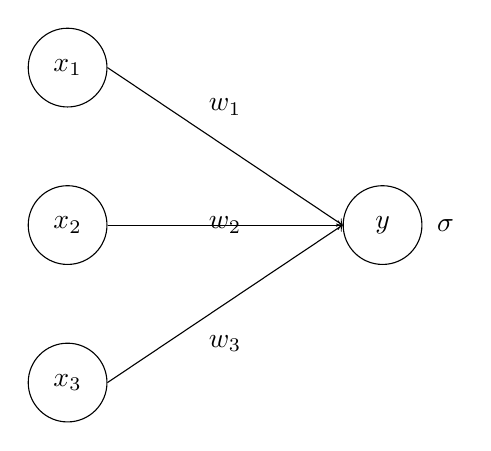
\begin{tikzpicture}[scale=1.0, transform shape]

        % Nodos de entrada
        \node[circle, draw, minimum size=1cm] (x1) at (0, 2) {$x_1$};
        \node[circle, draw, minimum size=1cm] (x2) at (0, 0) {$x_2$};
        \node[circle, draw, minimum size=1cm] (x3) at (0, -2) {$x_3$};
        
        % Nodo de salida
        \node[circle, draw, minimum size=1cm] (y) at (4, 0) {$y$};
        
        % Pesos (etiquetas)
        \node at (2, 1.5) {$w_1$};
        \node at (2, 0) {$w_2$};
        \node at (2, -1.5) {$w_3$};
        
        % Conexiones
        \draw[->] (x1.east) -- (y.west);
        \draw[->] (x2.east) -- (y.west);
        \draw[->] (x3.east) -- (y.west);
        
        %
        \node at (4.8, 0) {$\sigma$};

    \end{tikzpicture}
    \caption{Ejemplo de perceptrón}
    \label{fig:perceptron}
\end{figure}




\begin{definition}[Capa]
Sea $\mathbf{W} \in \mathbb{R}^{n\times m}$ una matriz de pesos, $\mathbf{h} \in \mathbb{R}^n$ un vector de entradas (resultado de la salida de una capa anterior) y $\mathbf{b} \in \mathbb{R}^n$ un vector de bias, $\sigma : \mathbb{R} \longrightarrow \mathbb{R}$ una función de activación.
La capa L-ésima $f^{(L)}$ de una red neuronal, está definida por:

\[
f^{(L)} = \sigma \circ \mathbf{h}^{(L)}
\]

Donde:
\begin{itemize}
    \item $\mathbf{h}^{(L)}$ = $\mathbf{W}^{(L)}f^{(L-1)}+b^{(i)}$ es la combinación lineal entre la matriz de pesos $\mathbf{W}$ que conecta la capa $L$ con la capa $L-1$ y la salida de la capa anterior.
    \item $\sigma(\cdot)$ es la función de activación.
    \item $\mathbf{h}^{(0)} = \mathbf{X}$ tal que $\mathbf{X} \in \mathbb{R}^{d}$, con $d$ el número de entradas.
    
\end{itemize}


\end{definition}


\begin{definition}[Red Neuronal]
Una \textbf{Red Neuronal} con $\boldmath{\mathbf{L}}$ capas es la composición de las funciones $f_i$ , $i \in \{1, \dotsc , \mathbf{L}\}$ tales que:

\[y = f(x;\theta) = f^{(\mathbf{L})}(f^{(\mathbf{L}-1)}(\dotsc f^{(2)}(f^{(1)}(x))))\]
Donde:
\begin{itemize}
    \item $\mathbf{x}$ es el vector de entrada.
    \item $f_i$ es la transformación realizada por la capa i-ésima.
    \item $\theta$ son los paramétros de la red (pesos y bias).
    \item $\mathbf{y}$ es la salida.
\end{itemize}    
\end{definition}

\begin{definition}[Función de pérdida]
Sea $y$ el valor verdadero del resultado de una tarea de aprendizaje,$\hat{y} = f(x;\theta)$
una red neuronal,entonces la función de pérdida \[\mathbf{L}(y,\hat{y})\]
mide la diferencia entre ambos, valor verdadero y valor predicho, donde el objetivo es encontrar los parametros $\theta$ que minimicen dicha función, es decir:
\[ \underset{\theta}{\textbf{min}} \frac{1}{N}\sum_{i=1}^N L(y_i,f(x_i;\theta))\]
\begin{example}
La función de pérdida puede variar dependiendo de la tarea que se realice, aquí tenemos una serie de ejemplo de dicha función dependiendo del contexto
\begin{itemize}
    \item \textbf{Error cuadrático medio (MSE)}\\
    Esta función de pérdida es comúnmente usada en problemas de regresión.Mide la diferencia entre lso valores $y$, $\hat{y}$ elevando al cuadrado dicha diferencia:
    \[L(y,\hat{y}) = \frac{1}{N} \sum_{i=1}^{N}(y_i - \hat{y}_i)^2\]
\item \textbf{Error absoluto medio (MAE)}\\
Utilizada también para tareas de regresión que mide la magnitud de los erores de manera más robusta, se define como:
\[
L(y, \hat{y}) = \frac{1}{N} \sum_{i=1}^{N}|y_i - \hat{y}_i|
\]
\item \textbf{Entropía cruzada}\\
Esta función es utilizada habitualmente en problemas de clasificación midiendo la similitud entre la probabildad predicha $\hat{y}$ y la real $y$, de forma generalizada para $\mathbf{K}$ número de clases se tiene que:
\[
L(y,\hat{y}) = - \sum_{i=1}^{K}y_ilog(\hat{y}_i)
\]
\end{itemize}
\end{example}


    
\end{definition}

\begin{definition}[Función de riesgo]
Sea $\mathbf{X}$ el vector de características de entrada y sea $\mathbf{y}$ la variable objetivo, dada la red neuronal $f(x;\theta)$ la función de riesgo se define cómo:

\[
\mathcal{R}(\theta) = \mathbb{E}[\mathbf{L}(y,f(x;\theta))]
\]
Donde:
\begin{itemize}
    \item $\mathbb{E}$ es  la esperanza de la distribución conjunta ($\mathbf{x}$,$\mathbf{y}$).
    \item $\mathbf{L}(y,f(x;\theta))$ es la función de pérdida, entre $y$ , $f(x;\theta)$
\end{itemize}
\end{definition}

Dado que en la práctica no conocemos la verdadera distribución $p(x,y)$ no podemos calcular directamente el riesgo esperado.En su lugar definimos otro tipo de función de riesgo:
\begin{definition}[Función de riesgo empírico]
Sea $\{(x_i,y_i)\}, i \in\{1,\cdots,N\}$ un conjunto finito de datos de entrenamiento, la función de riesgo empírico está dada por:

\[
\hat{\mathcal{R}}(\theta) = \frac{1}{N} \sum_{i=1}^{N} \mathbf{L} ( y_i,f(x_i;\theta)
)
\]    
\end{definition}
Una manera de minimizar las funciones de pérdida, es utilizando el algoritmno de Gradiente Descendente.

\begin{definition}[Gradiente]
Sea $f: \Omega \subset \mathbb{R}^n \longrightarrow \mathbb{R}$,una función diferenciable en $x_0$.Entonces el vector cuyas compnentes son las derivadas parciales de $f$ en $x_0$ es el vector gradiente, denotado por $\nabla f$, donde:

\[\nabla f(x_0) = \left( \frac{\partial f(x_0)}{\partial x_1},\dotsc , \frac{\partial f(x_0)}{\partial x_n} \right)\]
\end{definition}
Este vector contiene la información de cuanto crece o decrece la función en un punto en específico.

\begin{definition}[Descenso por gradiente]
Sea $J: \Theta \longrightarrow \mathbb{R}$ una función objetivo, donde $\Theta$ es el espacio de soluciones, $\eta$ la tasa de aprendizaje del modelo que determina el tamaño de los pasos en cada iteración, entonces,
se define al gradiente descendente cómo un método para encontrar el mínimo de una función de forma iterativa, se basa en iterar los valores de $\theta$ en la dirección negativa del gradiente de $J(\theta)$ de la siguiente forma:

\[
\theta \leftarrow \theta - \eta \nabla_\theta J(\theta)
\] 
\end{definition}
A continuación definiremos el algortimo que se utiliza para la actualización de los valores $\theta$ utilizando el gradiente descendente:
\begin{algorithm}
\caption{Algoritmo de actualización GD}\label{alg:cap}
\begin{algorithmic}
\Inputs{ $J:\Theta \longrightarrow \mathbb{R}$, $\mathbf{T} > 0$ número de iteraciones, $\eta$ rango de aprendizaje.}
\Initialize{Seleccionar $\theta ^ {(0)} \in \Theta$ aleatoriamente.}
\For{$t \in \{1,\dotsc,\mathbf{T}\}$}
\State Calcular $R(\theta ^{(t)})$, $\nabla_{\theta^{(T)}}R(\theta ^{(t)})$
\If{$\nabla_{\theta^{(T)}}R(\theta ^{(t)}) \neq$  0}
\State $\theta ^{(t+1)} \gets \theta^{(t)} - \eta \nabla_{\theta^{(t)}}R(\theta ^{(t)})$
\Else
\State Fin del algoritmo
\EndIf
\EndFor
\end{algorithmic}
\end{algorithm}
\noindent Existen otras variantes del Descenso de Gradiente, pero para efectos de esta tesis, nos quedaremos con la definición más básica.
A medida que va aumentando el número de capas en la red neuronal, también aumenta la complejidad de determinar los pesos de todas las conexiones de manera correcta para minimizar los errores, es por eso que nace la necesidad de implementar algoritmos más complejos para la optimización de redes multicapa, de ahí que nace el \textbf{BackPropagation}.
(Pendiente)
\begin{definition}[Derivada función de riesgo]
Sea $f(x;\theta)$ una red neuronal con parametros $\theta$, la derivada de su función de riesgo $R(\theta)$ se define de la siguiente forma:
\[
\nabla_\theta R(\theta) = \nabla f^{(\mathbf{L})} \cdot \nabla f^{(\mathbf{L}-1)} \cdots \nabla f^{(2)} \cdot \nabla f^{(1)} 
\]
\end{definition}
Notamos que esta definición es posible gracias a la regla de la cadena.

(anexo)
\begin{observation}[Propagación hacia adelante]
Ya sabemos que para cada capa $(L)$ de una red neuronal, la salida $\mathbf{h}^{(L)}$ se calcula de manera recursiva, dado un vector de entrada $\mathbf{x}$ la red realiza las siguientes dos operaciones:

\begin{itemize}
    \item \textbf{Preactivación} \\
    Dada la matriz de pesos $\mathbf{W}^{(L)}$ , el vector de sesgos $\mathbf{b}^(L)$ en la capa $L$ y $\mathbf{h}^(L-1)$ la salida de la capa anterior, entonces la preactivación está dada por: 
    \[
    \mathbf{z}^{(L)} = \mathbf{W}^{(L)}\mathbf{h}^{(L-1)} + \mathbf{b}^{(L)}
    \]
    \item \textbf{Activación}\\
    Dada $\sigma$ una función de activación (sigmoide,ReLu,etc), y $\mathbf{z}^{(L)}$ la preactivación de la capa $L$, entonces la activación en la capa $L$ está dada por:
    \[
    \mathbf{h}^{(L)} = \sigma \left( \mathbf{z}^{(L)} \right)
    \]
\end{itemize}
De esta forma la salida de la última capa se compara con la etiqueta verdadera $y$ utilizando alguna función de pérdida $\mathbf{J}(\mathbf{h}^{(L)},y)$
\end{observation}

\begin{observation}[Minimización del error en la capa de salida]\
Para minimizar el error en la función de pérdida utilizamos la definición 32, por una serie de pasos dados de la siguiente manera:
\begin{itemize}
    \item \textbf{Error en la capa de salida}\\
    Sea $\frac{\partial \mathbf{J}}{\partial \mathbf{h}^{(L)}} $ el gradiente de la función de pérdida con respecto a la salida de la red, $\sigma ' (\mathbf{z}^{(L)})$, la derivada de la función de activación de la última capa, entonces el error en la capa de salida está dado por:
    \[
    \delta^{(L)} = \frac{\partial \mathbf{J}}{\partial \mathbf{z}^{(L)}} = \frac{\partial \mathbf{J}}{\partial \mathbf{h}^{(L)}} \cdot \sigma ' (z^{(L)})
    \]
    \item \textbf{Propagación del error hacía atrás}\\
        Sea $\delta ^{(L+1)}$ el error de la capa siguiente y $\sigma ' (z^{(L)})$ la derivada de la función de activación de la capa L, entonces la propagación del error se da mediante la siguiente expresión: 
        \[
        \delta^{(L)} = \left( W^{(L+1)}\right)^T \delta ^{(L+1)} \cdot \sigma ' (z^(L)) 
        \]
    \item \textbf{Gradiente de los parámetros}\\
    Para calcular los gradientes de los parametros, vemos que se realiza de la siguiente forma:
    \begin{itemize}
        \item Sea $h^{(L-1)}$ la salida de la capa anterior, entonces el gradiente de los pesos está dado por: 
        \[
        \frac{\partial \mathbf{J}}{\partial \mathbf{    W}^{(L)}} = \delta ^{(L)} \cdot \left(a^{(L-1)}\right)^T
        \]
        \item Y para los sesgos se calcula de la siguiente forma:
        \[
        \frac{\partial\mathbf{J}}{\partial b^{(L)}} = \delta^{(L)}
        \]
    \end{itemize}
    
    \item \textbf{Actualización de los parámetros}\\
    Una vez que se tienen los pesos y sesgos calculados de la red, se actualizan utilizando un método de optimización ya mencionado anteriormente llamado descenso del gradiente, de esta forma la actualización está dada por: 
    \begin{itemize}
        \item \textbf{Pesos}:
        \[
        W^{(L)} = W^{(L)}- \eta \frac{\partial \mathbf{J}}{\partial W^{(L)}}
        \]
        
        \item \textbf{Bias}:
        \[
        b^{(L)} = b^{(L)}- \eta \frac{\partial\mathbf{J}}{\partial b^{(L)}}
        \]
        
    \end{itemize}
    
\end{itemize}

\end{observation}
Con lo observado anteriormente, podemos definir el algoritmo \textbf{backpropagation} enunciado en el siguiente pseudocódigo:

\begin{algorithm}
\caption{Algoritmo Backpropagation}
\begin{algorithmic}[1]
    \State \textbf{Initialize} Inicializamos pesos $W^{[l]}$ y bias $b^{[l]}$ de manera aleatoria para cada capa $l = 1, \dots, L$
    
    \For{cada época}
        \For{cada ejemplo de entrenamiento $(x, y)$}
        
            \State \textbf{Propagación hacía adelante}:
            \State Asignamos $a^{[0]} = x$
            \For{each layer $l = 1, \dots, L$}
                \State $z^{[l]} = W^{[l]} a^{[l-1]} + b^{[l]}$
                \State $a^{[l]} = g(z^{[l]})$
            \EndFor
            
            \State \textbf{Calculamos la pérdida} $J(a^{[L]}, y)$
            
            \State \textbf{Backward Pass}:
            \State Calculamos el error para cada capa de salida:
            \State $\delta^{[L]} = \frac{\partial J}{\partial a^{[L]}} \cdot g'(z^{[L]})$
            
            \For{cada capa $l = L-1, \dots, 1$}
                \State Propagación del error hacía atrás:
                \State $\delta^{[l]} = (W^{[l+1]})^\top \delta^{[l+1]} \cdot g'(z^{[l]})$
                \State Calculamos los gradientes:
                \State $\frac{\partial J}{\partial W^{[l]}} = \delta^{[l]} \cdot (a^{[l-1]})^\top$
                \State $\frac{\partial J}{\partial b^{[l]}} = \delta^{[l]}$
            \EndFor
            
            \State \textbf{Actualización de parámetros} (Descenso del gradiente):
            \For{each layer $l = 1, \dots, L$}
                \State $W^{[l]} = W^{[l]} - \eta \cdot \frac{\partial J}{\partial W^{[l]}}$
                \State $b^{[l]} = b^{[l]} - \eta \cdot \frac{\partial J}{\partial b^{[l]}}$
            \EndFor
            
        \EndFor
    \EndFor
    
\end{algorithmic}
\end{algorithm}
Así, hemos definido los componentes de una red neuronal, su forma de optimización y su entrenamiento.
\newpage
\subsection{Redes convolucionales CNN}
Las \textbf{redes neuronales convolucionales (CNN)} son una clase especializada de redes neuronales diseñadas para procesar datos que poseen una estructura de malla o grilla, como imágenes y series de tiempo. Estas redes se emplean comúnmente en tareas de procesamiento de imágenes, donde los datos se organizan en una malla bidimensional, o en el caso de las series temporales, que pueden representarse como una malla unidimensional con muestras tomadas a lo largo de intervalos de tiempo.

A diferencia de las redes neuronales tradicionales, donde se utiliza la multiplicación general de matrices, las CNN aplican la operación de convolución en al menos una de sus capas. Esto les permite extraer automáticamente características locales de los datos, como bordes, texturas o patrones, lo que mejora significativamente su capacidad para procesar datos con una estructura espacial clara.

Estudiar las CNN es fundamental como antecedente para entender las redes gráficas convolucionales (GCN), ya que comparten la idea central de la convolución, pero aplicadas a estructuras de datos más complejas, como los grafos. En esta sección, exploraremos la importancia de las CNN como base teórica, profundizando en su arquitectura y en las matemáticas que subyacen a este tipo particular de redes.La mayoría de las definiciones fueron obtenidas del libro \cite{Goodfellow-et-al-2016}.
\begin{definition}[Convolución]
Sean $x,w$ : $\mathbb{R} \longrightarrow \mathbb{R}$ dos funciones. La convolución de $x$ y $w$ denotada por: $(x \ast w)(t)$ es una operación binaria que produce una nueva función dada por:
\[
s(t) = (x \ast w)(t) = \int x(a)w(t-a)da
\]
    
\end{definition}
En el contexto de las redes neuronales convolucionales, el primer término (la función $x$) se refiere a la entrada, y el segundo término (la función $w$) es el kernel o filtro.
Dado que en muchos escenarios, el tipo de datos es discreto, se maneja otro tipo de convolución, llamda convolución dicreta.
\begin{definition}[Convolución discreta]
Sean $x(n)$,$w(n)$ dos sucesiones, la convolución discreta, se define como:
 \[
 (x \ast w)(n) = \sum _{a = - \infty}^{\infty} x(n)w(n-a)
 \]
    
\end{definition}
Finalmente, para el uso particular del procesamiento de imágenes en dos dimensiones, podemos utilizar la convolución discreta en dos dimensiones.
\begin{definition}[Convolución en dos dimensiones]
Sean $\mathbf{I}$ y $\mathbf{K}$ dos matrices definidas en $\mathbf{M}_{22}$, la convolución de matrices discretas se define cómo:
\[
\mathbf{S}(i,j) = (\mathbf{I} \ast \mathbf{K})(i,j) = \sum_{m} \sum_{n} \mathbf{I}(m,n) \mathbf{K}(i-m,j-n)
\]
\begin{observation}
    Notamos que, como la convolución es conmutativa, entonces la definición anterior puede reescribirse de tal forma que:
    \[
    \mathbf{S}(i,j) = (\mathbf{K} \ast \mathbf{I})(i,j) = \sum_{m} \sum_{n} \mathbf{I}(i-m.j-n)\mathbf{K}(m,n)    
    \]
\end{observation}
     
\end{definition}
\begin{definition}[Kernel (Filtro)]
Sea $\mathbf{X} \in \mathbb{R}^{m\times n}$ un conjunto de datos de entrada.El kernel (o filtro) $\mathbf{K}$ es una matriz de pesos de tamaño $h \times w$ donde $m \geq h, n \geq w$. Tal que actúa sobre la entrada $\mathbf{X}$ mediante una convolución, es decir:
\[
(\mathbf{K} \ast \mathbf{X})(i,j) = \sum_{u=1}^{h} \sum_{v=1}^{w} \mathbf{X}(i+u-1,j+v-1)\mathbf{K}(u,v)
\]    
Donde se introduce el término -1 para alinear el kernel con la entrada de manera que este quede centrado.
\end{definition}

\begin{center}
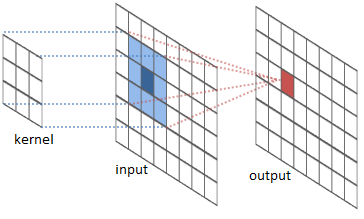
\includegraphics[scale=0.6]{img/conv_illustration.png}

    
\end{center}

A continuación, enunciaremos algunas propiedas clave de los filtros.
\begin{definition}[Propiedades del kernel]
Sea $\mathbf{K}$ un filtro de dimensiones $h \times w$.
\begin{itemize}
    \item \textbf{Dimensión} 
    La dimensión del kernel está dado por: 
    \[ dim(\mathbf{K}) = h \times w\]
    \item \textbf{Simetría}
    Un kernel es simétrico si satisface: 
    \[
    \mathbf{K}(i,j) = \mathbf{K}(h-i,w-j) \hspace{1cm} \forall \hspace{5pt} i,j \in \{0,\cdots,h\},\{0, \cdots,w\}
    \]
    \item \textbf{Normalización}
    Se dice que un kernel está normalizado si :
    \[
    \sum_{i=0}^h \sum_{j=0}^w \mathbf{K}(i,j)=1
    \]
\end{itemize}

\end{definition}

\begin{definition}[Mapa de características]
Sea $\mathbf{I}$ un tensor de entrada, $\mathbf{K}$ el kernel, el mapa de características $\mathbf{F}$está dado por:
\[
\mathbf{F}(i,j)=(\mathbf{I} \ast \mathbf{K})(i,j)
\]

    
\end{definition}
\begin{definition}[Stride]
Sea $\mathbf{K}$ un filtro de tamaño $h \times w$ aplicado en una entrada $\mathbf{I}$, entonces el stride $\mathbf{s}$ para cada entrada $i,j$ está determinado por:
\[
(i \cdot s, j \cdot s)
\]
por lo cual el mapa de características quedaría determinado por : \[
\mathbf{F}(l,m) = \mathbf{F}(i\cdot s,j\cdot s) \hspace{1cm} l=i \cdot s, m = j\cdot s
\]
\end{definition}
\begin{definition}[Padding]
Sea $\mathbf{I}$ una entrada de dimensiones $m \times n$ el padding $\mathbf{p}$ de tamaño $\rho$  es una función $\mathbf{p}_{\rho} : \mathbb{R}^{m \times n} \longrightarrow \mathbb{R}^{(m+2 \rho) \times (n+2 \rho)}$ tal que: 
\[
\mathbf{p}_\rho(\mathbf{I})(i, j) = 
\begin{cases} 
\alpha, & \text{si } i \leq \rho \text{ , } j \leq \rho \text{ , } i > m + \rho \text{ , } j > n + \rho \\ 
\mathbf{I}(i - \rho, j - \rho), & \text{en otro caso}.
\end{cases}
\]
Donde $\alpha \in \mathbb{R}$.

    
\end{definition}
 \begin{definition}[Invarianza]
 Sea $f: \mathbf{X} \longrightarrow \mathbf{Y}$ una función, $\mathbf{T}$ una transformación en $\mathbf{X}$. Se dice que una función $f$ es invariante bajo $\mathbf{T}$ si:
 \[
 f\left(\mathbf{T}(x)\right) = f(x) , \hspace{1cm} \forall x \in \mathbf{X}
 \]
 \end{definition}

 \begin{definition}[Equivarianza]
 Sean $f,g$ dos funciones tales que $f: \mathbf{X} \longrightarrow \mathbf{Y}$, $g : \mathbf{Y} \longrightarrow \mathbf{X}$. Se dice que $f$ es equivariante bajo $g$ si:
 \[
 f\left( g(x)\right) = g\left(f(x)\right) \hspace{1cm} \forall x \in \mathbf{X}
 \]
     
 \end{definition}
 De las definiciones anteriores, podemos notar que están muy relacionadas ya que al aplicar convoluciones a datos estructurados podemos notar que tiene la propiedad de ser equivariante con respecto a ciertas transformaciones, por ejemplo a la traslación.

 \begin{observation}
     Sea $f$ una función y consideremos la trasnformación $\mathbf{T}_a$ cómo la traslación de su entrada en la cantidad a, es decir: $\mathbf{T}_af(x) = f(x-a)$.
     Aplicando la convolución tenemos que:
     \[
     (\mathbf{T}_af \ast k)(x) = \int_{\mathbb{R}} \mathbf{T}_af(t)k(x-t)dt
     \]
     Sustituyendo el valor de la transformación obtenemos:
     \[
     (\mathbf{T}_af \ast k)(x) = \int_{\mathbb{R}} f(t-a)k(x-t)dt
     \]
     Y realizando el cambio de variable $u = t-a$ tenemos que $du = dt$ y además $t=u+a$ así:
     \[
     (\mathbf{T}_af \ast k)(x) =
     \int_{\mathbb{R}} f(u)k(x-(u+a))du
     \]
     Que, reordenando los términos obtenemos lo siguiente:
     \[
     (\mathbf{T}_af \ast k)(x) =
     \int_{\mathbb{R}} f(u)k((x-a)-u)du
     \]
     Que por definición tenemos que: 
     \[
     (f \ast k)(x-a) = 
     \int_{\mathbb{R}} f(u)k((x-a)-u)du
     \]
     Por lo tanto:
     \[
     (\mathbf{T}_af \ast k)(x) = (f \ast k)(x-a) \hspace{1cm} \forall x \in \mathbb{R}
     \]
 \end{observation}
 De esta forma, demostramos que la operación convolución para funciones definidas en $\mathbb{R}$ son equivariantes con respecto a las traslaciones.
 Es decir , que en el contexto de las redes neuronales, si trasladamos la entrada de la red, significa que la salida estará traslada en la misma medida, lo cual es útil cuando se aplica a múltiples ubicaciones en la entrada.

 \begin{definition}[Max Pooling]
 Sea $\mathbf{X}$ una entrada en $\mathbb{R}^{m \times n}$, $\mathbf{s}$ un stride dado, $\mathbf{M}: \mathbb{R}^{m \times n} \longrightarrow \mathbb{R}^{p \times q}$ una función, entonces la función $\mathbf{M}$ está dada por:
 \[
 \mathbf{M}(\mathbf{X})(i,j) = \max_{0 \leq u < h , 0 \leq v < w} \mathbf{X}(i\cdot s + u,j\cdot s+v)
 \]   
 \end{definition}

 \begin{definition}[Average pooling]
 Sea $\mathbf{X}$ una entrada en $\mathbb{R}^{m \times n}$, $\mathbf{s}$ un stride dado, $\mathbf{A}: \mathbb{R}^{m \times n} \longrightarrow \mathbb{R}^{p \times q}$ una función, entonces la función $\mathbf{A}$ está dada por:
 \[
 \mathbf{A}(\mathbf{X})(i,j) = \frac{1}{h \cdot w} \sum_{u=0}^{h-1}\sum_{v=0}^{w-1} \mathbf{X}(i\cdot s + u, j \cdot s + v)
 \]
\end{definition}
Hasta ahora, se ha visto como las operaciones de convolución y pooling extraen las características de una red neuronal, una vez realizadas estas operaciones, el resultado se aplana en un único vector con el objetivo de utilizado como entrada para una capa completamente conectada donde se realizará la tarea que se requiera.

\begin{definition}[Arquitectura de una CNN]
Sea $f: \mathbb{R}^{m \times n \times d} \longrightarrow \mathbb{R}^k$ una función, la arquitectura de una red neuronal convolucional (CNN) se define como la composición de tres funciones donde la composición está dad por:
\[
\mathbf{y} = \mathbf{g} \circ \mathbf{P} \circ \mathbf{C}(\mathbf{X})
\]
donde:

\begin{itemize}
    \item $\mathbf{C(\mathbf{X}) = (\mathbf{K} \ast \mathbf{X}) + \mathbf{b}}$
    es la capa convolucional.
    \item $\mathbf{P(\mathbf{C}(\mathbf{X}))} = \max_{0 \leq u < h , 0 \leq v < w} \mathbf{C}(\mathbf{X}(i\cdot s + u,j\cdot s+v))$
    Representa la capa de pooling y para este caso, como ejemplo se utiliza el máx pooling.
    \item $\mathbf{y} = g(\mathbf{W}\mathbf{P} + \mathbf{b})$ es la capa completamente conectada.
\end{itemize}

\end{definition}
\newpage
\subsection{Redes Neuronales Gráficas}

\begin{definition}[Encoder]
Sea $G$ una gráfica,un encoder es una función $\phi$ tal que $\phi: \mathcal{V} \longrightarrow \mathbb{R}^d$ dada por:
\[
\phi(v,\mathcal{N}(v),G(E)) = z_v \hspace{1cm} donde \hspace{5pt} z_v\in \mathbb{R}^d
\]
\end{definition}
Por simplicidad denotaremos $\phi(v,\mathcal{N}(v),E(v)) :=\phi(v)$
\begin{definition}[Matriz de encajes]
Sea $v \in \mathcal{V}$ tenemos que:
\[
\phi(v) = \mathbf{Z}[v] \hspace{1cm} donde \hspace{5pt} \mathbf{Z} \in \mathbb{R}^{ \nu_{G}\times d}
\] es una matriz que contiene los vectores de encajes $z_v$ correspondientes a cada nodo de la gráfica.
    
\end{definition}

\begin{definition}[Decoder]
Sea $z_v \in \mathbb{R}^d$ un encaje producido por un encoder,entonces la función $\psi:\mathbb{R}^d \longrightarrow Y$ se denomina decoder, y produce una prediccón en el espacio de salida $Y$, es decir:
\[
\psi(z_v) = \hat{y}
\]
\end{definition}

Pointnet tiene una parte de encoder y deceoder

\subsection{Propagación de Mensajes Neuronales}
El concepto de \textbf{Propagación de Mensajes Neuronales} se refiere al mecanismo mediante el cual las representaciones de los vértices de una gráfica, se actualizan mediante el intercambio de información de su vecindario.
En cada paso del mecanismo, los nodos intercambian mensajes que contienen información sobre el estado en que se encuentran para luego combinarse y actualizar su información interna.\\
Esto viene motivado por la necesidad de capturar relaciones y dependencias entre los vértices de una gráfica para estudiar su comportamiento estructural.\\
En diferentes contextos del mundo actual, notamos que muchos de los datos tienen una estructura propia de gráfica, tales como: redes sociales, moléculas, sistemas de recomendación, etc, siendo los vértices entidades como usuarios,átomos o productos de un e-commerce y las aristas las relaciones entre ellos tales como, amistades,enlaces y preferencias.
El concepto de \textbf{Propagación de Mensajes Neuronales}, permite estudiar a la gráfica, no sólo a nivel de característica de vértice, sino también a nivel estructural de gráfica.\\

\begin{center}

\includegraphics{Example-of-a-message-passing-neural-network-The-left-side-is-an-example-of-a-graphical}

    
\end{center}


\subsection{Descripción general del mecanismo}
\noindent Cómo se mencionó en la motivación, durante cada iteración del mecanismo en una GNN (Red Neuronal Gráfica), los encajes ocultos $h_u^{(k)}$ correspondientes a cada nodo $u \in V$, son actualizadas de acuerdo a la información recopilada del vecinadrio de $u$.

El mecanismo puede ser definido de la siguiente forma:
\begin{definition}[Propagación de mensajes neuronales]
Sea , $G=(V,E)$ una gráfica, $N_G(v)$ el vecindario del nodo $v \in V$ y $h_u^{(t)}$los encajes ocultos del nodo $v$, y $\mathscr{A}$ una función de agregación que combina los encajes  de los vecinos de $v$ entonces, el mecanismo de propagación de mensajes está dado por:
\[
m_v^{(t)} = \mathscr{A}(h_u^{(k)})
\]
    
\end{definition}
Una vez que el vértice a recibido el mensaje, la actualización de su información es el resultado de la combinación del mensaje recibido, con la información actual que tenía y se define de la siguiente forma:
\begin{definition}
    Sea $h_v^{(t-1)}$ el encaje oculto de la capa anterior $(t-1)$, y $m_v^{(t)}$ la propagación del mensaje en la capa $t$, entonces la actualización del mensaje está dado por:
    \[
    h_v^{(t)} = \mathscr{U} (h_v^{(t-1)},m_v^{(t)})
    \]
    Donde $\mathscr{U}$ es una función de actualización, normalmente es una red neuronal, con una capa lineal seguida de una función de activación (ReLu)
\end{definition}

Después de K iteraciones del mecanismo, podemos utilizar la salida del final de la capa para definir los encajes de cada vértice, es decir:

\begin{center}
    $z_u$ = $h_u^{(K)}$.
\end{center}

\subsection{La GNN fundamental}
Hasta el momento, se ha estudiado el marco de las GNN de una manera un poco abstracta utilizando las funciones que definimos en la sección anterior e iterando K veces.\\
Para introducir una manera de abordarlas de forma más general, introducimos el modelo GNN más básico.
El modelo GNN fundamental es definido por:

    \[h_u =  \phi\left(x_u, \bigoplus_{v \in \mathcal{N}(u)}
   \psi(x_u,x_v)    \right)\]
Donde:

\begin{itemize}
    \item $h_u$ es la nueva representación del nodo $u$ después de aplicar una capa de la GNN
    \item $x_u$ Representa la característica del nodo $u$ antes de la actualización.
    \item $\psi(x_u,x_v)$ Es una función de transformación que toma las características del nodo $u$ y de su vecino $v$,produciendo una especie de mensaje o interacción entre ambos nodos.
    \item $\bigoplus_{v \in \mathcal{N}(u)}$ Es una operación de agregación como puede ser suma,media, max pooling,etc, sobre los vecinos de $u$ es decir sobre las transformaciones producidas por la función $\psi(\cdot)$.
    \item $\phi(\cdot)$ es la función de actualización que toma las características originales del nodo $u (x_u)$ y el resultado de la agregación de los mensajes de sus vecinos para producir una nueva representación del nodo $u$.
\end{itemize}

En términos generales, el comportamiento lo podemos describir a continuación:

\begin{enumerate}
    \item \textbf{Mensajes entre nodos vecinos} ($\psi(x_u,x_v)$)\\
    La función \boldmath{$\psi$} calcula la interacción entre las características del nodo $u$ y las caracterísiticas de cada unos de sus vecinos $v$.Esto permite capturar la relación entre los nodos de forma que dependa de sus características.\\
    \item \textbf{Agregación} ($\bigoplus$)\\
    Después de calcular las interacciones entre $u$ y sus vecinos, estas interacciones se agregan mediante una operación $\bigoplus$, que cómo comúnmente (cómo se vió anteriormente) es una suma, media o máximo.La agregación tiene comoobjetivo combinar toda la información recibida entre los vecinos de $u$ en un solo término.
    \item \textbf{Actualización}($\phi$)\\
    Finalmente, la función $\phi$ toma la característica original del nodo $u$,$x_u$ y el resultado de la agregación para producir la nueva representación $h_u$.La función $\phi$ puede ser una red neuronal feedforward o cualquier otra transformación no lineal que aprenda a integrar la información de $u$ con la de sus vecinos.
   
\end{enumerate}
En resumen, el modelo anterior expresa el proceso de \textbf{message passing} de una GNN,donde los mensajes de los vecinos de un nodo se combinan para actualizar la representación del nodo central,aprovechando las simetrías presentes en las gráficas.
\subsection{Redes Gráficas Convolucionales (GCNs)}

\begin{definition}Arquitectura de una GNN]
Sea $G$ una gráfica, $A$ su matriz de adyacencia $\mathbf{F}$ una función de activación, $\Phi$ los parámetros de la red, entonces la arquitectura de una GCN está definida por:
\begin{align*} 
\mathbf{H}_1 &=  \mathbf{F}[\mathbf{X},\mathbf{A},\Phi_0] \\ 
\mathbf{H}_2 &=  \mathbf{F}[\mathbf{H}_!,\mathbf{A},\Phi_1]\\
\vdots &= \vdots \\
\mathbf{H}_K &= \mathbf{F}[\mathbf{H}_{K-1},\mathbf{A},\Phi_{K-1}]
\end{align*}
Donde $\mathbf{X}$ es la entrada y $\mathbf{H}_K$ contiene los encajes de nodos modificados.
\end{definition}

\begin{definition}[Equivarianza]
Sea $\mathbf{F}$ una función de activación $\mathbf{H}$ la matriz de encajes ocultos de nodos, $\mathbf{P}$ una matriz de permutación, decimos que una capa es equivariante si:
\[
\mathbf{H}_{K+1}\mathbf{P}= \mathbf{F}[\mathbf{H}_K \mathbf{P},\mathbf{P}^T\mathbf{A}\mathbf{P},\Phi_K]
\]
Donde $A$ es la matriz de adyacencia para la gráfica $G$
    
\end{definition}

Pointnet utiliza equivarianza y lo podemos mostrar.
No importa la gráfica 